\newpage
 \thispagestyle{endchapter}
\begin{tcolorbox}
	\vspace{80pt}
	\lettrine{W}{e} left \passage{Primadona} after focussing on the shallow leads ICCC had started to explore in 2016. While our main efforts concentrated on three pushing fronts (\passage{Déj Vu}, \passage{Electric Dreams} and \passage{Fenestrator}), short reconnaissance trips and resurvey projects raised the possibility of a new underground camp closer to the old Slovenian pushing front, at -600m. 
	
	On a particular exchange trip between the \passage{TTT} and \passage{Karstaway} branches, three possible sites were spotted; it will be the goal of the forthcoming year to determine which is most suitable for the objective of `bottoming' the cave at last. 

	To throw spanners in the works, the eleventh-hour extension of \passage{Hallelujah} streamway to \passage{Sweet Baby Jesus}, an the pitch series of Alabaster contributed to shifting the aims and expectations of future expeditions. 
	
	It now seems certain that at least part of the motivation for exploring \passage{Primadona} will be down to the awaiting, half-descended pitch, hovering above blank mountain. Time will tell whether it will prove key to unlocking yet another of the Hollow Mountain's secrets.
	
	\mydelimiter
	
	\begin{quote} The time to prepare for your next expedition is when you have just returned from a successful trip. 
	
	 \name{Robert Peary} \end{quote}

\end{tcolorbox}

	\backgroundsetup{	scale=1,
					color=black,
					opacity=1,
					angle=270,
					contents={%
  							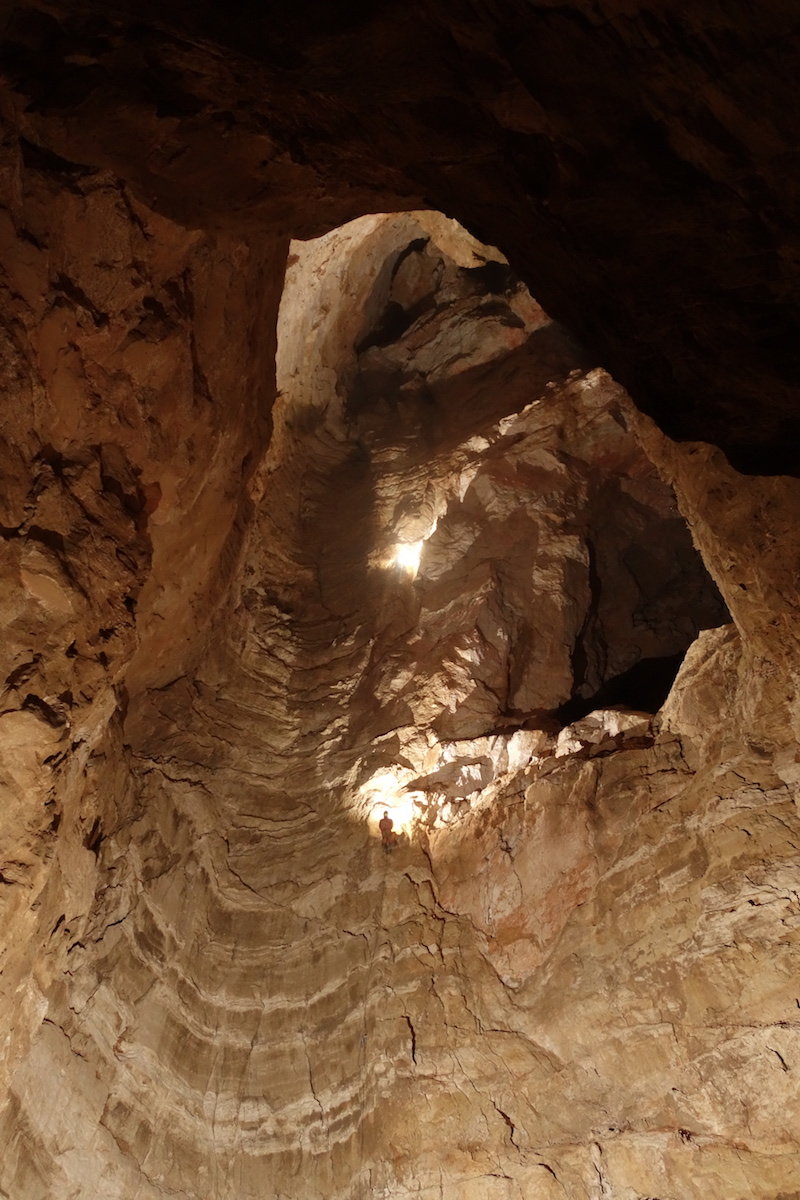
\includegraphics[width=\paperwidth, angle=90]{images/backgrounds/galaktika-rhys.jpg}
  					}
	}
\BgThispage

